% Options for packages loaded elsewhere
\PassOptionsToPackage{unicode}{hyperref}
\PassOptionsToPackage{hyphens}{url}
%
\documentclass[
]{article}
\usepackage{lmodern}
\usepackage{amsmath}
\usepackage{ifxetex,ifluatex}
\ifnum 0\ifxetex 1\fi\ifluatex 1\fi=0 % if pdftex
  \usepackage[T1]{fontenc}
  \usepackage[utf8]{inputenc}
  \usepackage{textcomp} % provide euro and other symbols
  \usepackage{amssymb}
\else % if luatex or xetex
  \usepackage{unicode-math}
  \defaultfontfeatures{Scale=MatchLowercase}
  \defaultfontfeatures[\rmfamily]{Ligatures=TeX,Scale=1}
\fi
% Use upquote if available, for straight quotes in verbatim environments
\IfFileExists{upquote.sty}{\usepackage{upquote}}{}
\IfFileExists{microtype.sty}{% use microtype if available
  \usepackage[]{microtype}
  \UseMicrotypeSet[protrusion]{basicmath} % disable protrusion for tt fonts
}{}
\makeatletter
\@ifundefined{KOMAClassName}{% if non-KOMA class
  \IfFileExists{parskip.sty}{%
    \usepackage{parskip}
  }{% else
    \setlength{\parindent}{0pt}
    \setlength{\parskip}{6pt plus 2pt minus 1pt}}
}{% if KOMA class
  \KOMAoptions{parskip=half}}
\makeatother
\usepackage{xcolor}
\IfFileExists{xurl.sty}{\usepackage{xurl}}{} % add URL line breaks if available
\IfFileExists{bookmark.sty}{\usepackage{bookmark}}{\usepackage{hyperref}}
\hypersetup{
  pdftitle={Forecasting DTC},
  pdfauthor={Glen Lewis, Jonathan Burns, Eric Beekman, Andrew Nalundasan},
  hidelinks,
  pdfcreator={LaTeX via pandoc}}
\urlstyle{same} % disable monospaced font for URLs
\usepackage[margin=1in]{geometry}
\usepackage{color}
\usepackage{fancyvrb}
\newcommand{\VerbBar}{|}
\newcommand{\VERB}{\Verb[commandchars=\\\{\}]}
\DefineVerbatimEnvironment{Highlighting}{Verbatim}{commandchars=\\\{\}}
% Add ',fontsize=\small' for more characters per line
\usepackage{framed}
\definecolor{shadecolor}{RGB}{248,248,248}
\newenvironment{Shaded}{\begin{snugshade}}{\end{snugshade}}
\newcommand{\AlertTok}[1]{\textcolor[rgb]{0.94,0.16,0.16}{#1}}
\newcommand{\AnnotationTok}[1]{\textcolor[rgb]{0.56,0.35,0.01}{\textbf{\textit{#1}}}}
\newcommand{\AttributeTok}[1]{\textcolor[rgb]{0.77,0.63,0.00}{#1}}
\newcommand{\BaseNTok}[1]{\textcolor[rgb]{0.00,0.00,0.81}{#1}}
\newcommand{\BuiltInTok}[1]{#1}
\newcommand{\CharTok}[1]{\textcolor[rgb]{0.31,0.60,0.02}{#1}}
\newcommand{\CommentTok}[1]{\textcolor[rgb]{0.56,0.35,0.01}{\textit{#1}}}
\newcommand{\CommentVarTok}[1]{\textcolor[rgb]{0.56,0.35,0.01}{\textbf{\textit{#1}}}}
\newcommand{\ConstantTok}[1]{\textcolor[rgb]{0.00,0.00,0.00}{#1}}
\newcommand{\ControlFlowTok}[1]{\textcolor[rgb]{0.13,0.29,0.53}{\textbf{#1}}}
\newcommand{\DataTypeTok}[1]{\textcolor[rgb]{0.13,0.29,0.53}{#1}}
\newcommand{\DecValTok}[1]{\textcolor[rgb]{0.00,0.00,0.81}{#1}}
\newcommand{\DocumentationTok}[1]{\textcolor[rgb]{0.56,0.35,0.01}{\textbf{\textit{#1}}}}
\newcommand{\ErrorTok}[1]{\textcolor[rgb]{0.64,0.00,0.00}{\textbf{#1}}}
\newcommand{\ExtensionTok}[1]{#1}
\newcommand{\FloatTok}[1]{\textcolor[rgb]{0.00,0.00,0.81}{#1}}
\newcommand{\FunctionTok}[1]{\textcolor[rgb]{0.00,0.00,0.00}{#1}}
\newcommand{\ImportTok}[1]{#1}
\newcommand{\InformationTok}[1]{\textcolor[rgb]{0.56,0.35,0.01}{\textbf{\textit{#1}}}}
\newcommand{\KeywordTok}[1]{\textcolor[rgb]{0.13,0.29,0.53}{\textbf{#1}}}
\newcommand{\NormalTok}[1]{#1}
\newcommand{\OperatorTok}[1]{\textcolor[rgb]{0.81,0.36,0.00}{\textbf{#1}}}
\newcommand{\OtherTok}[1]{\textcolor[rgb]{0.56,0.35,0.01}{#1}}
\newcommand{\PreprocessorTok}[1]{\textcolor[rgb]{0.56,0.35,0.01}{\textit{#1}}}
\newcommand{\RegionMarkerTok}[1]{#1}
\newcommand{\SpecialCharTok}[1]{\textcolor[rgb]{0.00,0.00,0.00}{#1}}
\newcommand{\SpecialStringTok}[1]{\textcolor[rgb]{0.31,0.60,0.02}{#1}}
\newcommand{\StringTok}[1]{\textcolor[rgb]{0.31,0.60,0.02}{#1}}
\newcommand{\VariableTok}[1]{\textcolor[rgb]{0.00,0.00,0.00}{#1}}
\newcommand{\VerbatimStringTok}[1]{\textcolor[rgb]{0.31,0.60,0.02}{#1}}
\newcommand{\WarningTok}[1]{\textcolor[rgb]{0.56,0.35,0.01}{\textbf{\textit{#1}}}}
\usepackage{graphicx}
\makeatletter
\def\maxwidth{\ifdim\Gin@nat@width>\linewidth\linewidth\else\Gin@nat@width\fi}
\def\maxheight{\ifdim\Gin@nat@height>\textheight\textheight\else\Gin@nat@height\fi}
\makeatother
% Scale images if necessary, so that they will not overflow the page
% margins by default, and it is still possible to overwrite the defaults
% using explicit options in \includegraphics[width, height, ...]{}
\setkeys{Gin}{width=\maxwidth,height=\maxheight,keepaspectratio}
% Set default figure placement to htbp
\makeatletter
\def\fps@figure{htbp}
\makeatother
\setlength{\emergencystretch}{3em} % prevent overfull lines
\providecommand{\tightlist}{%
  \setlength{\itemsep}{0pt}\setlength{\parskip}{0pt}}
\setcounter{secnumdepth}{-\maxdimen} % remove section numbering
\ifluatex
  \usepackage{selnolig}  % disable illegal ligatures
\fi

\title{Forecasting DTC}
\author{Glen Lewis, Jonathan Burns, Eric Beekman, Andrew Nalundasan}
\date{November 18, 2021}

\begin{document}
\maketitle

{
\setcounter{tocdepth}{3}
\tableofcontents
}
+Forecasting Housing Prices

Housing price growth has exploded in recent months and house prices in
general have increased from 1975 onward. It has become vital to lenders,
individuals, and government officials to monitor changes in house prices
over time to appropriately plan for home ownership and changes in
housing affordability at scale. We specifically wanted to investigate
how house proces have changed in the last decade and compare
pre-pandemic to post-pandemic price changes.

+Data Description

We used the Freddie Mac House Price Index (FMPHI) available at
\url{http://www.freddiemac.com/research/indices/house-price-index.page}.

Per the Freddie Mac website ``the FMHPI provides a measure of typical
price inflation for houses within the United States. Values are
calculated monthly and released at the end of the following month. For
example, the FMHPI for March is published in late April.'' The data
includes seasonally and non-seasonally adjusted series which are
available at three different geographical levels (metropolitan, state,
and national)for each month going all the way back to January 1975.

For our forecasting analysis we split the data into 3 sections based on
the changes in the graph of NSA index over time. There is the
2011-presnet section and we then identified 2011-2019 as pre-pandemic
and 2020-2021 as post-pandemic.

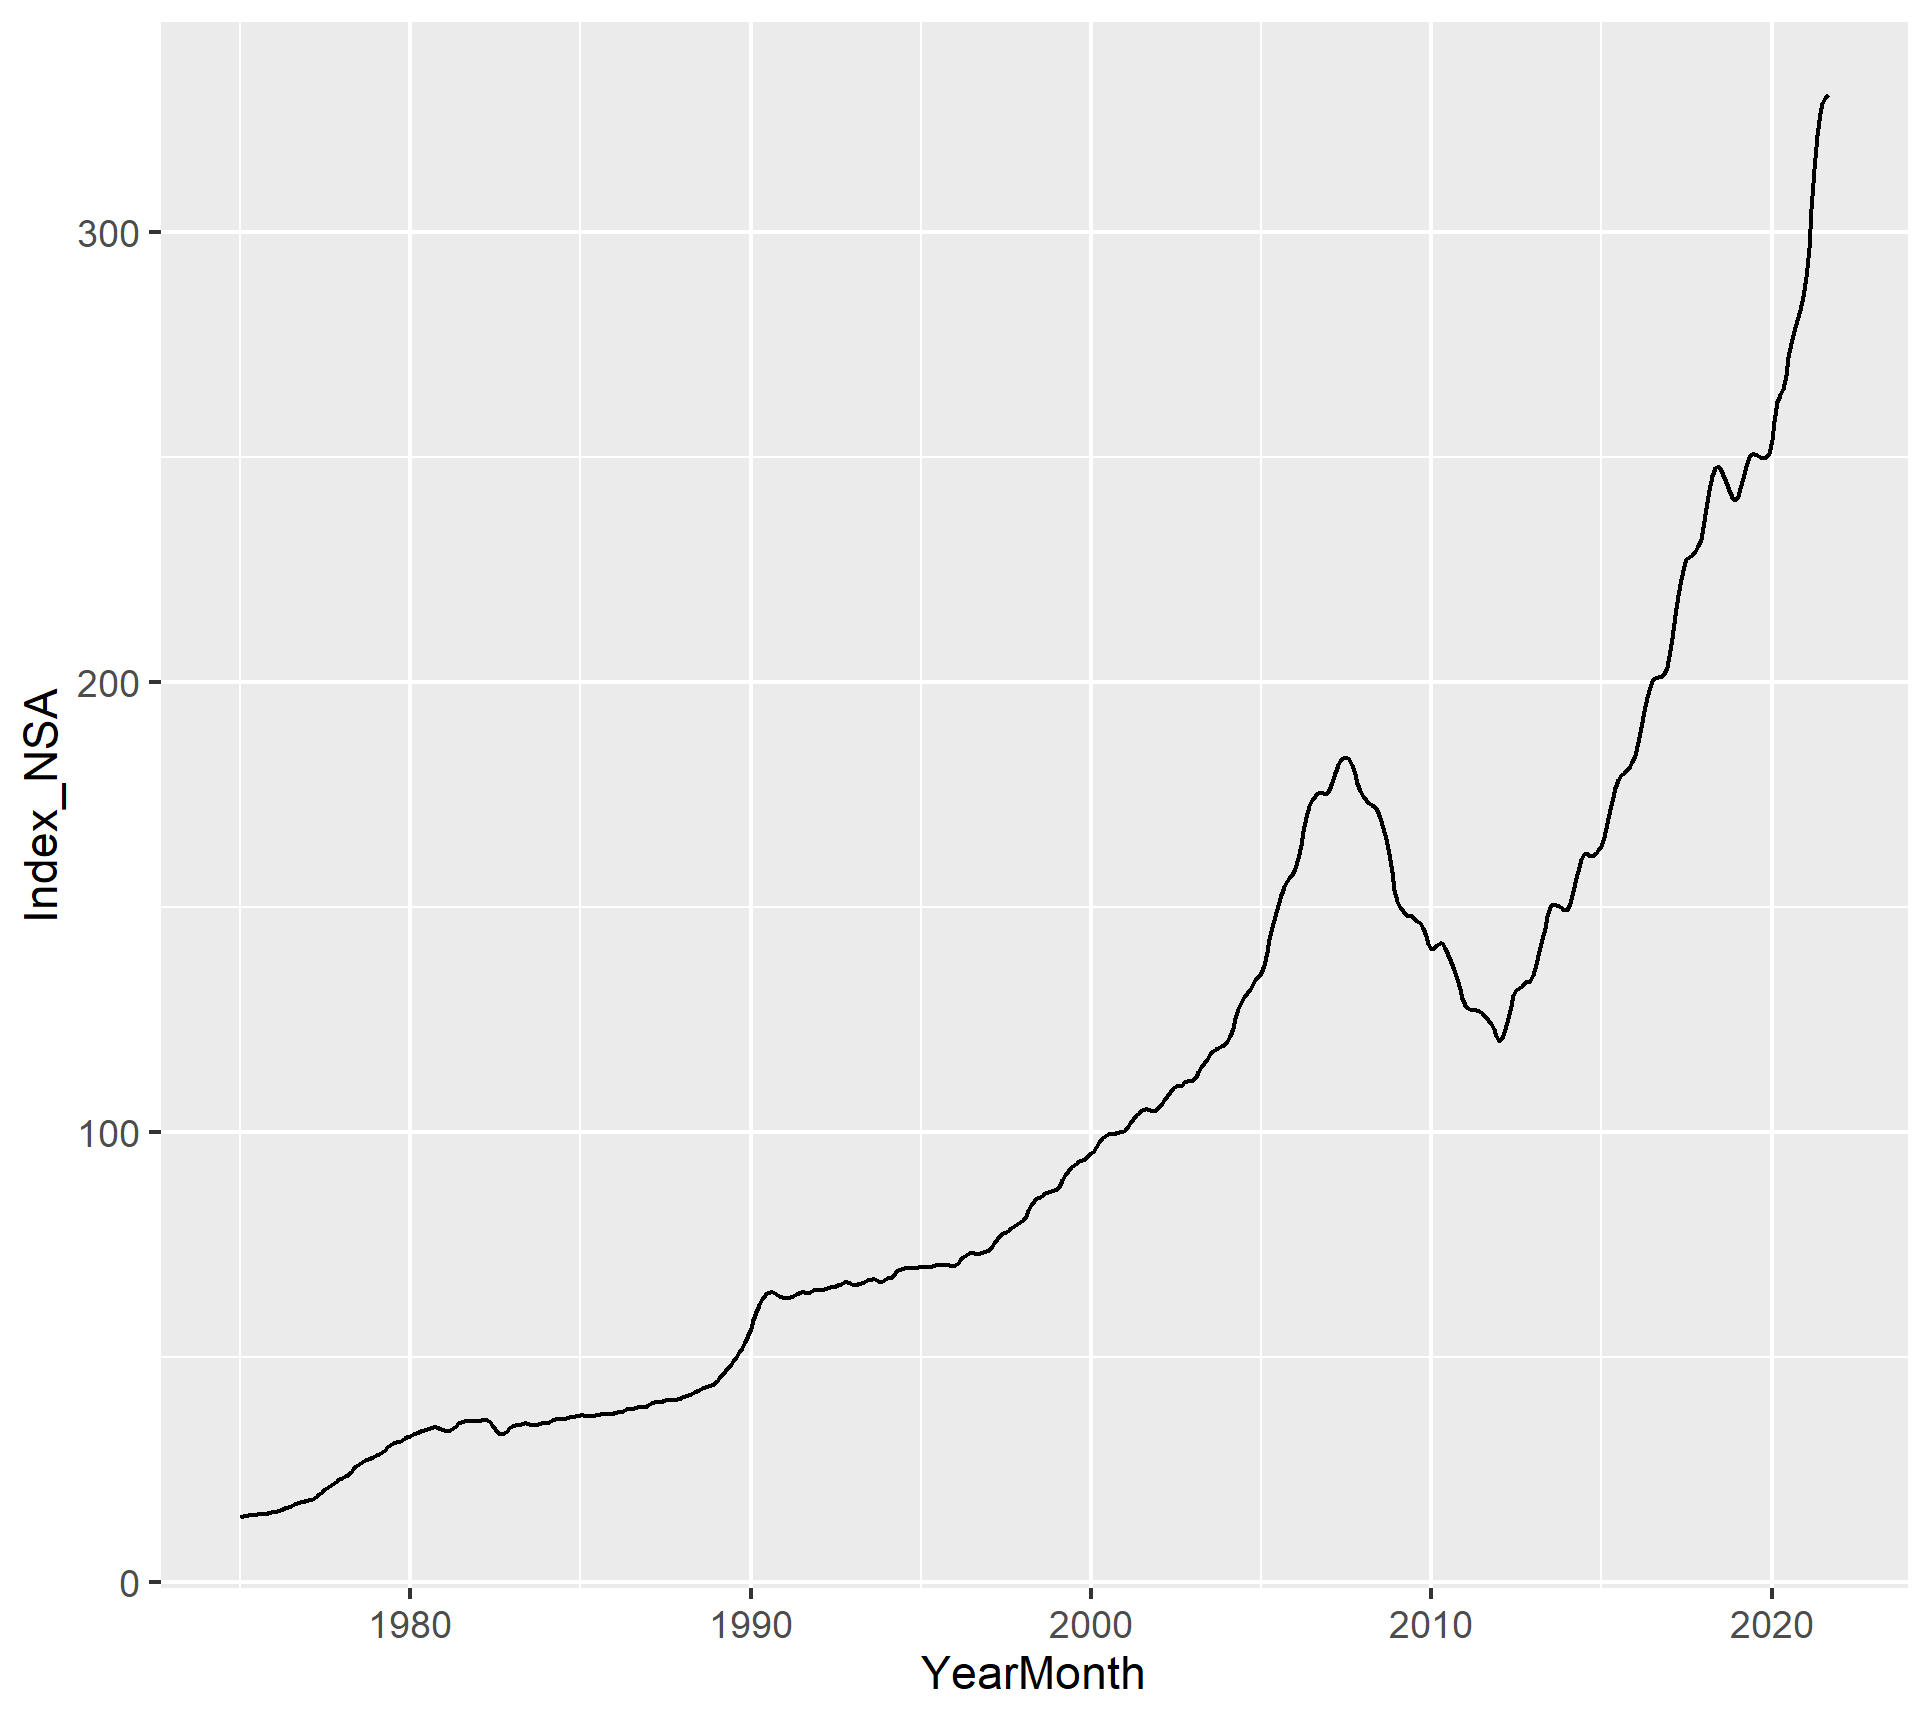
\includegraphics[width=5.20833in,height=5.20833in]{NSA-graph.png}

\hypertarget{read-in-data-and-wrangle}{%
\section{Read in data and wrangle}\label{read-in-data-and-wrangle}}

\begin{Shaded}
\begin{Highlighting}[]
\CommentTok{\# read in data}
\NormalTok{data }\OtherTok{\textless{}{-}} \FunctionTok{read\_csv}\NormalTok{(}\StringTok{"../02\_raw\_data/fmhpi\_master\_file.csv"}\NormalTok{)}
\end{Highlighting}
\end{Shaded}

\begin{verbatim}
## 
## -- Column specification --------------------------------------------------------
## cols(
##   Year = col_double(),
##   Month = col_double(),
##   GEO_Type = col_character(),
##   GEO_Name = col_character(),
##   GEO_Code = col_character(),
##   Index_NSA = col_double(),
##   Index_SA = col_double()
## )
\end{verbatim}

\begin{Shaded}
\begin{Highlighting}[]
\CommentTok{\# look at the data}
\FunctionTok{head}\NormalTok{(data, }\DecValTok{10}\NormalTok{)}
\end{Highlighting}
\end{Shaded}

\begin{verbatim}
## # A tibble: 10 x 7
##     Year Month GEO_Type GEO_Name GEO_Code Index_NSA Index_SA
##    <dbl> <dbl> <chr>    <chr>    <chr>        <dbl>    <dbl>
##  1  1975     1 State    AK       .             34.4     34.6
##  2  1975     2 State    AK       .             34.9     35.0
##  3  1975     3 State    AK       .             35.3     35.4
##  4  1975     4 State    AK       .             35.9     35.7
##  5  1975     5 State    AK       .             36.5     36.2
##  6  1975     6 State    AK       .             37.2     36.7
##  7  1975     7 State    AK       .             37.9     37.2
##  8  1975     8 State    AK       .             38.6     37.9
##  9  1975     9 State    AK       .             39.2     38.6
## 10  1975    10 State    AK       .             39.7     39.4
\end{verbatim}

\begin{Shaded}
\begin{Highlighting}[]
\CommentTok{\# filter for target GEO}
\NormalTok{puget }\OtherTok{\textless{}{-}}\NormalTok{ data }\SpecialCharTok{\%\textgreater{}\%} 
  \FunctionTok{filter}\NormalTok{(GEO\_Type }\SpecialCharTok{==} \StringTok{\textquotesingle{}CBSA\textquotesingle{}}\NormalTok{, GEO\_Name }\SpecialCharTok{==} \StringTok{\textquotesingle{}Seattle{-}Tacoma{-}Bellevue WA\textquotesingle{}}\NormalTok{)}
\end{Highlighting}
\end{Shaded}

\begin{verbatim}
## filter: removed 242,913 rows (>99%), 561 rows remaining
\end{verbatim}

\begin{Shaded}
\begin{Highlighting}[]
\NormalTok{puget}\SpecialCharTok{$}\NormalTok{YearMonth }\OtherTok{\textless{}{-}} \FunctionTok{as.Date}\NormalTok{(}\FunctionTok{with}\NormalTok{(puget, }\FunctionTok{paste}\NormalTok{(Year, Month, }\DecValTok{1}\NormalTok{, }\AttributeTok{sep=}\StringTok{"{-}"}\NormalTok{)),}\StringTok{"\%Y{-}\%m{-}\%d"}\NormalTok{)}

\NormalTok{puget\_nsa }\OtherTok{\textless{}{-}}\NormalTok{ puget[, }\FunctionTok{c}\NormalTok{(}\StringTok{\textquotesingle{}YearMonth\textquotesingle{}}\NormalTok{, }\StringTok{\textquotesingle{}Index\_NSA\textquotesingle{}}\NormalTok{)] }\SpecialCharTok{\%\textgreater{}\%} 
  \FunctionTok{filter}\NormalTok{(YearMonth }\SpecialCharTok{\textgreater{}=} \StringTok{\textquotesingle{}2011{-}01{-}01\textquotesingle{}}\NormalTok{)}
\end{Highlighting}
\end{Shaded}

\begin{verbatim}
## filter: removed 432 rows (77%), 129 rows remaining
\end{verbatim}

\begin{Shaded}
\begin{Highlighting}[]
\NormalTok{puget\_sa }\OtherTok{\textless{}{-}}\NormalTok{ puget[, }\FunctionTok{c}\NormalTok{(}\StringTok{\textquotesingle{}YearMonth\textquotesingle{}}\NormalTok{, }\StringTok{\textquotesingle{}Index\_SA\textquotesingle{}}\NormalTok{)] }\SpecialCharTok{\%\textgreater{}\%} 
  \FunctionTok{filter}\NormalTok{(YearMonth }\SpecialCharTok{\textgreater{}=} \StringTok{\textquotesingle{}2011{-}01{-}01\textquotesingle{}}\NormalTok{)}
\end{Highlighting}
\end{Shaded}

\begin{verbatim}
## filter: removed 432 rows (77%), 129 rows remaining
\end{verbatim}

\begin{Shaded}
\begin{Highlighting}[]
\CommentTok{\# declare as TS}
\NormalTok{puget\_nsa\_ts }\OtherTok{\textless{}{-}} \FunctionTok{ts}\NormalTok{(puget}\SpecialCharTok{$}\NormalTok{Index\_NSA, }\AttributeTok{frequency=}\DecValTok{12}\NormalTok{, }\AttributeTok{start=}\DecValTok{1975}\NormalTok{)  }\CommentTok{\# monthly data}

\NormalTok{puget\_sa\_ts }\OtherTok{\textless{}{-}} \FunctionTok{ts}\NormalTok{(puget}\SpecialCharTok{$}\NormalTok{Index\_SA, }\AttributeTok{frequency=}\DecValTok{12}\NormalTok{, }\AttributeTok{start=}\DecValTok{1975}\NormalTok{)  }\CommentTok{\# monthly data}
\end{Highlighting}
\end{Shaded}

\begin{itemize}
\item
  Data wrangling:

  \begin{itemize}
  \tightlist
  \item
    filter geography for `Seattle-Tacoma-Bellevue WA'
  \item
    create new column for `YearMonth' concatenating to be \%Y-\%m-\%d
    format
  \item
    filter dataset to be dates from 2011-present for research question 1
  \end{itemize}
\end{itemize}

\hypertarget{research-question-1-forecasting-from-2011-present}{%
\section{Research Question 1: Forecasting from
2011-present}\label{research-question-1-forecasting-from-2011-present}}

\begin{Shaded}
\begin{Highlighting}[]
\CommentTok{\# plot TS}
\FunctionTok{plot}\NormalTok{(puget\_nsa, }\AttributeTok{col=}\StringTok{\textquotesingle{}blue\textquotesingle{}}\NormalTok{, }\AttributeTok{main=}\StringTok{\textquotesingle{}Seattle, Tacoma, Bellevue}\SpecialCharTok{\textbackslash{}n}\StringTok{Non{-}Seasonally Adjusted index trends\textquotesingle{}}\NormalTok{, }\AttributeTok{ylab=}\StringTok{\textquotesingle{}Non{-}Seasonally Adjusted Index\textquotesingle{}}\NormalTok{, }\AttributeTok{xlab=}\StringTok{\textquotesingle{}Year\textquotesingle{}}\NormalTok{)}
\end{Highlighting}
\end{Shaded}

\includegraphics{DTC_code_AN_files/figure-latex/unnamed-chunk-3-1.pdf}

\begin{Shaded}
\begin{Highlighting}[]
\FunctionTok{plot}\NormalTok{(puget\_sa, }\AttributeTok{col=}\StringTok{\textquotesingle{}blue\textquotesingle{}}\NormalTok{, }\AttributeTok{main=}\StringTok{\textquotesingle{}Seattle, Tacoma, Bellevue}\SpecialCharTok{\textbackslash{}n}\StringTok{Non{-}Seasonally Adjusted index trends\textquotesingle{}}\NormalTok{, }\AttributeTok{ylab=}\StringTok{\textquotesingle{}Seasonally Adjusted Index\textquotesingle{}}\NormalTok{, }\AttributeTok{xlab=}\StringTok{\textquotesingle{}Year\textquotesingle{}}\NormalTok{)}
\end{Highlighting}
\end{Shaded}

\includegraphics{DTC_code_AN_files/figure-latex/unnamed-chunk-3-2.pdf}

\begin{Shaded}
\begin{Highlighting}[]
\CommentTok{\# plot histogram}
\FunctionTok{hist}\NormalTok{(puget\_nsa\_ts)}
\end{Highlighting}
\end{Shaded}

\includegraphics{DTC_code_AN_files/figure-latex/unnamed-chunk-3-3.pdf}

\begin{Shaded}
\begin{Highlighting}[]
\FunctionTok{hist}\NormalTok{(puget\_sa\_ts)}
\end{Highlighting}
\end{Shaded}

\includegraphics{DTC_code_AN_files/figure-latex/unnamed-chunk-3-4.pdf}

\textbf{Comments}

\begin{itemize}
\tightlist
\item
  Need to take difference to achieve stationarity
\end{itemize}

\begin{Shaded}
\begin{Highlighting}[]
\CommentTok{\# log difference of puget}
\NormalTok{ld\_puget\_nsa }\OtherTok{\textless{}{-}} \FunctionTok{diff}\NormalTok{(}\FunctionTok{log}\NormalTok{(puget\_nsa\_ts))}
\NormalTok{ld\_puget\_sa }\OtherTok{\textless{}{-}} \FunctionTok{diff}\NormalTok{(}\FunctionTok{log}\NormalTok{(puget\_sa\_ts))}

\CommentTok{\# plot the logged difference datasets}
\FunctionTok{plot}\NormalTok{(ld\_puget\_nsa, }\AttributeTok{col=}\StringTok{\textquotesingle{}blue\textquotesingle{}}\NormalTok{, }\AttributeTok{main=}\StringTok{\textquotesingle{}Seattle, Tacoma, Bellevue}\SpecialCharTok{\textbackslash{}n}\StringTok{Log Difference Index\_NSA trends\textquotesingle{}}\NormalTok{, }\AttributeTok{ylab=}\StringTok{\textquotesingle{}Non{-}Seasonally Adjusted Index\textquotesingle{}}\NormalTok{, }\AttributeTok{xlab=}\StringTok{\textquotesingle{}Year\textquotesingle{}}\NormalTok{)}
\end{Highlighting}
\end{Shaded}

\includegraphics{DTC_code_AN_files/figure-latex/unnamed-chunk-4-1.pdf}

\begin{Shaded}
\begin{Highlighting}[]
\FunctionTok{plot}\NormalTok{(ld\_puget\_sa, }\AttributeTok{col=}\StringTok{\textquotesingle{}blue\textquotesingle{}}\NormalTok{, }\AttributeTok{main=}\StringTok{\textquotesingle{}Seattle, Tacoma, Bellevue}\SpecialCharTok{\textbackslash{}n}\StringTok{Log Difference Index\_SA trends\textquotesingle{}}\NormalTok{, }\AttributeTok{ylab=}\StringTok{\textquotesingle{}Seasonally Adjusted Index\textquotesingle{}}\NormalTok{, }\AttributeTok{xlab=}\StringTok{\textquotesingle{}Year\textquotesingle{}}\NormalTok{)}
\end{Highlighting}
\end{Shaded}

\includegraphics{DTC_code_AN_files/figure-latex/unnamed-chunk-4-2.pdf}

\begin{Shaded}
\begin{Highlighting}[]
\CommentTok{\# create linear regression for time series data}
\CommentTok{\# model1 \textless{}{-} dynlm(dp \textasciitilde{} lag(dp, {-}1) + lag(dr, {-}1))}
\end{Highlighting}
\end{Shaded}

\textbf{Comments}

\begin{itemize}
\item
  After taking the log difference from the TS, does this yield a
  stationary trend?

  \begin{itemize}
  \tightlist
  \item
    This looks stationary but need to verify
  \end{itemize}
\item
  What does this tell us?
\end{itemize}

\begin{Shaded}
\begin{Highlighting}[]
\CommentTok{\# auto correlation function}
\CommentTok{\# 20 lags}
\FunctionTok{acf}\NormalTok{(puget\_nsa\_ts, }\AttributeTok{lag.max =} \DecValTok{20}\NormalTok{, }\AttributeTok{main=}\StringTok{\textquotesingle{}Puget NSA TS {-} ACF\textquotesingle{}}\NormalTok{)}
\end{Highlighting}
\end{Shaded}

\includegraphics{DTC_code_AN_files/figure-latex/Plot ACF-1.pdf}

\begin{Shaded}
\begin{Highlighting}[]
\FunctionTok{acf}\NormalTok{(puget\_sa\_ts, }\AttributeTok{lag.max =} \DecValTok{20}\NormalTok{, }\AttributeTok{main=}\StringTok{\textquotesingle{}Puget SA TS {-} ACF\textquotesingle{}}\NormalTok{)}
\end{Highlighting}
\end{Shaded}

\includegraphics{DTC_code_AN_files/figure-latex/Plot ACF-2.pdf}

\begin{Shaded}
\begin{Highlighting}[]
\CommentTok{\# see values only and no plot}
\FunctionTok{acf}\NormalTok{(puget\_nsa\_ts, }\AttributeTok{lag.max =} \DecValTok{20}\NormalTok{, }\AttributeTok{plot =} \ConstantTok{FALSE}\NormalTok{)}
\end{Highlighting}
\end{Shaded}

\begin{verbatim}
## 
## Autocorrelations of series 'puget_nsa_ts', by lag
## 
## 0.0000 0.0833 0.1667 0.2500 0.3333 0.4167 0.5000 0.5833 0.6667 0.7500 0.8333 
##  1.000  0.990  0.979  0.968  0.957  0.947  0.936  0.927  0.918  0.909  0.900 
## 0.9167 1.0000 1.0833 1.1667 1.2500 1.3333 1.4167 1.5000 1.5833 1.6667 
##  0.891  0.883  0.874  0.865  0.857  0.848  0.840  0.832  0.823  0.816
\end{verbatim}

\begin{Shaded}
\begin{Highlighting}[]
\FunctionTok{acf}\NormalTok{(puget\_sa\_ts, }\AttributeTok{lag.max =} \DecValTok{20}\NormalTok{, }\AttributeTok{plot =} \ConstantTok{FALSE}\NormalTok{)}
\end{Highlighting}
\end{Shaded}

\begin{verbatim}
## 
## Autocorrelations of series 'puget_sa_ts', by lag
## 
## 0.0000 0.0833 0.1667 0.2500 0.3333 0.4167 0.5000 0.5833 0.6667 0.7500 0.8333 
##  1.000  0.990  0.979  0.969  0.959  0.948  0.938  0.929  0.919  0.910  0.901 
## 0.9167 1.0000 1.0833 1.1667 1.2500 1.3333 1.4167 1.5000 1.5833 1.6667 
##  0.892  0.883  0.874  0.866  0.857  0.849  0.841  0.833  0.825  0.817
\end{verbatim}

\textbf{Comments}

\begin{itemize}
\item
  How many lags should we be running?
\item
  Arbitrarily chose 20 lags
\item
  Plot never falls below statistically significant threshold in 20 lags

  \begin{itemize}
  \tightlist
  \item
    PACF will likely fall below threshold before ACF
  \end{itemize}
\end{itemize}

\begin{Shaded}
\begin{Highlighting}[]
\CommentTok{\# PACF}
\FunctionTok{pacf}\NormalTok{(puget\_nsa\_ts, }\AttributeTok{lag.max =} \DecValTok{20}\NormalTok{, }\AttributeTok{main=}\StringTok{\textquotesingle{}Puget NSA TS {-} PACF\textquotesingle{}}\NormalTok{)}
\end{Highlighting}
\end{Shaded}

\includegraphics{DTC_code_AN_files/figure-latex/Plot PACF-1.pdf}

\begin{Shaded}
\begin{Highlighting}[]
\FunctionTok{pacf}\NormalTok{(puget\_sa\_ts, }\AttributeTok{lag.max =} \DecValTok{20}\NormalTok{, }\AttributeTok{main=}\StringTok{\textquotesingle{}Puget SA TS {-} PACF\textquotesingle{}}\NormalTok{)}
\end{Highlighting}
\end{Shaded}

\includegraphics{DTC_code_AN_files/figure-latex/Plot PACF-2.pdf}

\begin{Shaded}
\begin{Highlighting}[]
\CommentTok{\# values only}
\FunctionTok{pacf}\NormalTok{(puget\_nsa\_ts, }\AttributeTok{lag.max =} \DecValTok{20}\NormalTok{, }\AttributeTok{plot =} \ConstantTok{FALSE}\NormalTok{)}
\end{Highlighting}
\end{Shaded}

\begin{verbatim}
## 
## Partial autocorrelations of series 'puget_nsa_ts', by lag
## 
## 0.0833 0.1667 0.2500 0.3333 0.4167 0.5000 0.5833 0.6667 0.7500 0.8333 0.9167 
##  0.990 -0.018 -0.016 -0.009  0.004  0.016  0.021  0.020  0.011  0.001 -0.003 
## 1.0000 1.0833 1.1667 1.2500 1.3333 1.4167 1.5000 1.5833 1.6667 
## -0.005 -0.005 -0.003  0.000  0.005  0.004 -0.002  0.001  0.010
\end{verbatim}

\begin{Shaded}
\begin{Highlighting}[]
\FunctionTok{pacf}\NormalTok{(puget\_sa\_ts, }\AttributeTok{lag.max =} \DecValTok{20}\NormalTok{, }\AttributeTok{plot =} \ConstantTok{FALSE}\NormalTok{)}
\end{Highlighting}
\end{Shaded}

\begin{verbatim}
## 
## Partial autocorrelations of series 'puget_sa_ts', by lag
## 
## 0.0833 0.1667 0.2500 0.3333 0.4167 0.5000 0.5833 0.6667 0.7500 0.8333 0.9167 
##  0.990 -0.007 -0.008 -0.004  0.001  0.007  0.008  0.008  0.003  0.000  0.002 
## 1.0000 1.0833 1.1667 1.2500 1.3333 1.4167 1.5000 1.5833 1.6667 
##  0.004  0.004  0.005  0.006  0.009  0.003 -0.009 -0.010  0.000
\end{verbatim}

\textbf{Comments}

\begin{itemize}
\item
  PACF falls below statistically significant threshold at lag 2

  \begin{itemize}
  \tightlist
  \item
    This indicates that we are working with an Auto Regressive (AR)
    process
  \end{itemize}
\end{itemize}

\textbf{Questions}

\begin{itemize}
\item
  How many lags should we be running?

  \begin{itemize}
  \tightlist
  \item
    Arbitrarily chose 20 lags
  \end{itemize}
\item
  Does this indicate an ARIMA or ARMA model moving forward?
\item
  How do we determine what order of AR we are working with?

  \begin{itemize}
  \tightlist
  \item
    Perhaps once we determine a model?
  \end{itemize}
\end{itemize}

\begin{Shaded}
\begin{Highlighting}[]
\CommentTok{\# log difference of ACF and PACF}
\CommentTok{\# log difference ACF}
\FunctionTok{acf}\NormalTok{(ld\_puget\_nsa, }\AttributeTok{lag.max =} \DecValTok{20}\NormalTok{, }\AttributeTok{main =} \StringTok{\textquotesingle{}log diff Puget Sound Index\_NSA {-} ACF\textquotesingle{}}\NormalTok{)}
\end{Highlighting}
\end{Shaded}

\includegraphics{DTC_code_AN_files/figure-latex/unnamed-chunk-5-1.pdf}

\begin{Shaded}
\begin{Highlighting}[]
\FunctionTok{acf}\NormalTok{(ld\_puget\_sa, }\AttributeTok{lag.max =} \DecValTok{20}\NormalTok{, }\AttributeTok{main =} \StringTok{\textquotesingle{}log diff Puget Sound Index\_SA {-} ACF\textquotesingle{}}\NormalTok{)}
\end{Highlighting}
\end{Shaded}

\includegraphics{DTC_code_AN_files/figure-latex/unnamed-chunk-5-2.pdf}

\textbf{Comments}

\begin{itemize}
\tightlist
\item
  Coefficients don't drop below significance level until lag 5
\item
  Looks like a sinusoidal wave
\item
  Need to plot PACF logged difference
\end{itemize}

\begin{Shaded}
\begin{Highlighting}[]
\CommentTok{\# log difference PACF}
\FunctionTok{pacf}\NormalTok{(ld\_puget\_nsa, }\AttributeTok{lag.max =} \DecValTok{20}\NormalTok{, }\AttributeTok{main =} \StringTok{\textquotesingle{}log diff Puget Sound Index\_NSA {-} PACF\textquotesingle{}}\NormalTok{)}
\end{Highlighting}
\end{Shaded}

\includegraphics{DTC_code_AN_files/figure-latex/unnamed-chunk-6-1.pdf}

\begin{Shaded}
\begin{Highlighting}[]
\FunctionTok{pacf}\NormalTok{(ld\_puget\_sa, }\AttributeTok{lag.max =} \DecValTok{20}\NormalTok{, }\AttributeTok{main =} \StringTok{\textquotesingle{}log diff Puget Sound Index\_SA {-} PACF\textquotesingle{}}\NormalTok{)}
\end{Highlighting}
\end{Shaded}

\includegraphics{DTC_code_AN_files/figure-latex/unnamed-chunk-6-2.pdf}

\textbf{Comments}

\begin{itemize}
\item
  Oscillating coefficients indicate a negative number somewhere in the
  model or something like that
\item
  PACF drops below significance threshold at lag 5

  \begin{itemize}
  \tightlist
  \item
    Logged difference PACF indicates an AR process as well
  \item
    Is this enough evidence to confirm AR process?
  \item
    How can we verify via calculations?
  \end{itemize}
\end{itemize}

\textbf{Questions}

\begin{itemize}
\tightlist
\item
  These tests are just visual tests. How do we determine AR vs.~MA
  process computationally?
\end{itemize}

\hypertarget{following-arima-fitting-guide-using-ggplot}{%
\subsection{Following ARIMA fitting guide using
ggplot}\label{following-arima-fitting-guide-using-ggplot}}

\hypertarget{examine-data}{%
\subsubsection{Examine Data}\label{examine-data}}

\begin{Shaded}
\begin{Highlighting}[]
\CommentTok{\# plot using ggplot just for fun}
\FunctionTok{ggplot}\NormalTok{(puget, }\FunctionTok{aes}\NormalTok{(YearMonth, Index\_NSA)) }\SpecialCharTok{+} 
  \FunctionTok{geom\_line}\NormalTok{() }\SpecialCharTok{+} \FunctionTok{scale\_x\_date}\NormalTok{(}\StringTok{\textquotesingle{}Year\textquotesingle{}}\NormalTok{) }\SpecialCharTok{+} 
  \FunctionTok{labs}\NormalTok{(}\AttributeTok{y =} \StringTok{"Non{-}Seasonally Adjusted Index"}\NormalTok{,}
       \AttributeTok{title =} \StringTok{"Seattle, Tacoma, Bellevue"}\NormalTok{,}
       \AttributeTok{subtitle =} \StringTok{"Non{-}Seasonally Adjusted index trends"}\NormalTok{) }\SpecialCharTok{+}
  \FunctionTok{theme\_classic}\NormalTok{()}
\end{Highlighting}
\end{Shaded}

\includegraphics{DTC_code_AN_files/figure-latex/unnamed-chunk-7-1.pdf}

\textbf{Comments}

\begin{itemize}
\tightlist
\item
  ggplot plot looks exactly the same as using Base R but with more
  flexibility to add components
\item
  ggplot needs a DF rather than a TS to create plot
\end{itemize}

\begin{Shaded}
\begin{Highlighting}[]
\CommentTok{\# try cleaning the data}
\NormalTok{puget\_ts }\OtherTok{\textless{}{-}} \FunctionTok{ts}\NormalTok{(puget[, }\FunctionTok{c}\NormalTok{(}\StringTok{\textquotesingle{}Index\_NSA\textquotesingle{}}\NormalTok{)])}
\NormalTok{puget}\SpecialCharTok{$}\NormalTok{clean\_index\_nsa }\OtherTok{\textless{}{-}} \FunctionTok{tsclean}\NormalTok{(puget\_ts)}

\FunctionTok{ggplot}\NormalTok{() }\SpecialCharTok{+} 
  \FunctionTok{geom\_line}\NormalTok{(}\AttributeTok{data =}\NormalTok{ puget, }\FunctionTok{aes}\NormalTok{(}\AttributeTok{x =}\NormalTok{ YearMonth, }\AttributeTok{y =}\NormalTok{ clean\_index\_nsa)) }\SpecialCharTok{+} \FunctionTok{ylab}\NormalTok{(}\StringTok{\textquotesingle{}Cleaned Index NSA\textquotesingle{}}\NormalTok{)}
\end{Highlighting}
\end{Shaded}

\begin{verbatim}
## Don't know how to automatically pick scale for object of type ts. Defaulting to continuous.
\end{verbatim}

\includegraphics{DTC_code_AN_files/figure-latex/unnamed-chunk-8-1.pdf}

\textbf{Comments}

\begin{itemize}
\tightlist
\item
  cleaning the data using tsclean() does not have an effect on our
  dataset
\item
  no outliers to clean
\end{itemize}

\begin{Shaded}
\begin{Highlighting}[]
\CommentTok{\# plot the cleaned series}
\CommentTok{\# get MA(4) {-} quarterly MA}
\NormalTok{puget}\SpecialCharTok{$}\NormalTok{nsa\_ma04 }\OtherTok{=} \FunctionTok{ma}\NormalTok{(puget}\SpecialCharTok{$}\NormalTok{clean\_index\_nsa, }\AttributeTok{order=}\DecValTok{4}\NormalTok{) }\CommentTok{\# using the clean count with no outliers, get the MA}

\CommentTok{\# get MA(12) {-} yearly MA}
\NormalTok{puget}\SpecialCharTok{$}\NormalTok{nsa\_ma12 }\OtherTok{=} \FunctionTok{ma}\NormalTok{(puget}\SpecialCharTok{$}\NormalTok{clean\_index\_nsa, }\AttributeTok{order=}\DecValTok{12}\NormalTok{) }\CommentTok{\# MA(12)}

\FunctionTok{ggplot}\NormalTok{() }\SpecialCharTok{+} 
  \FunctionTok{geom\_line}\NormalTok{(}\AttributeTok{data =}\NormalTok{ puget, }\FunctionTok{aes}\NormalTok{(}\AttributeTok{x =}\NormalTok{ YearMonth, }\AttributeTok{y =}\NormalTok{ clean\_index\_nsa, }\AttributeTok{colour =} \StringTok{"Raw Data"}\NormalTok{)) }\SpecialCharTok{+}
  \FunctionTok{geom\_line}\NormalTok{(}\AttributeTok{data =}\NormalTok{ puget, }\FunctionTok{aes}\NormalTok{(}\AttributeTok{x =}\NormalTok{ YearMonth, }\AttributeTok{y =}\NormalTok{ nsa\_ma04,   }\AttributeTok{colour =} \StringTok{"Quarterly Moving Average"}\NormalTok{))  }\SpecialCharTok{+}
  \FunctionTok{geom\_line}\NormalTok{(}\AttributeTok{data =}\NormalTok{ puget, }\FunctionTok{aes}\NormalTok{(}\AttributeTok{x =}\NormalTok{ YearMonth, }\AttributeTok{y =}\NormalTok{ nsa\_ma12, }\AttributeTok{colour =} \StringTok{"Yearly Moving Average"}\NormalTok{))  }\SpecialCharTok{+}
  \FunctionTok{labs}\NormalTok{(}\AttributeTok{x =} \StringTok{"Year"}\NormalTok{, }
       \AttributeTok{y =} \StringTok{"NSA Index"}\NormalTok{,}
       \AttributeTok{title =} \StringTok{"Monthly MA vs. Weekly MA"}\NormalTok{) }\SpecialCharTok{+} 
  \FunctionTok{theme\_classic}\NormalTok{()}
\end{Highlighting}
\end{Shaded}

\begin{verbatim}
## Don't know how to automatically pick scale for object of type ts. Defaulting to continuous.
\end{verbatim}

\begin{verbatim}
## Warning: Removed 4 row(s) containing missing values (geom_path).
\end{verbatim}

\begin{verbatim}
## Warning: Removed 12 row(s) containing missing values (geom_path).
\end{verbatim}

\includegraphics{DTC_code_AN_files/figure-latex/unnamed-chunk-9-1.pdf}

\textbf{Comments}

\begin{itemize}
\tightlist
\item
  yearly MA appears to be a slightly smoother fit to our raw data plot
\item
  quarterly MA follows along almost spot on
\end{itemize}

\hypertarget{decompose-data}{%
\subsubsection{Decompose Data}\label{decompose-data}}

\begin{itemize}
\tightlist
\item
  Seasonality, Trend, Cycle to capture historical patterns in the series
\item
  Seasonality - fluctuations in the data related to calendar cycles
\item
  Trend - overall pattern of the series
\item
  Cycle - decreasing or increasing patterns that are not seasonal
\end{itemize}

\begin{Shaded}
\begin{Highlighting}[]
\CommentTok{\# Seasonality}
\NormalTok{nsa\_ma }\OtherTok{\textless{}{-}} \FunctionTok{ts}\NormalTok{(puget}\SpecialCharTok{$}\NormalTok{Index\_NSA, }\AttributeTok{frequency=}\DecValTok{12}\NormalTok{)}

\NormalTok{decomp }\OtherTok{\textless{}{-}} \FunctionTok{stl}\NormalTok{(nsa\_ma, }\AttributeTok{s.window=}\StringTok{"periodic"}\NormalTok{)  }\CommentTok{\# additive model structure}
\NormalTok{deseasonal\_nsa }\OtherTok{\textless{}{-}} \FunctionTok{seasadj}\NormalTok{(decomp)  }\CommentTok{\# remove seasonality}
\FunctionTok{plot}\NormalTok{(decomp)}
\end{Highlighting}
\end{Shaded}

\includegraphics{DTC_code_AN_files/figure-latex/unnamed-chunk-10-1.pdf}

\textbf{Comments}

\begin{itemize}
\tightlist
\item
  Not sure what this is telling us
\item
  why is time not in my time window?
\item
  definitely trending upwards
\end{itemize}

\hypertarget{stationarity}{%
\subsubsection{Stationarity}\label{stationarity}}

\begin{Shaded}
\begin{Highlighting}[]
\CommentTok{\# run ADF test}
\FunctionTok{adf.test}\NormalTok{(nsa\_ma, }\AttributeTok{alternative =} \StringTok{"stationary"}\NormalTok{)}
\end{Highlighting}
\end{Shaded}

\begin{verbatim}
## Warning in adf.test(nsa_ma, alternative = "stationary"): p-value greater than
## printed p-value
\end{verbatim}

\begin{verbatim}
## 
##  Augmented Dickey-Fuller Test
## 
## data:  nsa_ma
## Dickey-Fuller = 0.053668, Lag order = 8, p-value = 0.99
## alternative hypothesis: stationary
\end{verbatim}

\textbf{Comments}

\begin{itemize}
\tightlist
\item
  dickey-fuller test indicates a very high p-value
\item
  do these results indicate a stationary process?
\end{itemize}

\hypertarget{autocorrelations-and-choosing-model-order}{%
\subsubsection{Autocorrelations and Choosing Model
Order}\label{autocorrelations-and-choosing-model-order}}

\begin{Shaded}
\begin{Highlighting}[]
\CommentTok{\# plot ACF}
\FunctionTok{Acf}\NormalTok{(nsa\_ma, }\AttributeTok{main=}\StringTok{\textquotesingle{}ACF\textquotesingle{}}\NormalTok{)}
\end{Highlighting}
\end{Shaded}

\includegraphics{DTC_code_AN_files/figure-latex/unnamed-chunk-12-1.pdf}

\begin{Shaded}
\begin{Highlighting}[]
\CommentTok{\# plot PACF}
\FunctionTok{Pacf}\NormalTok{(nsa\_ma, }\AttributeTok{main=}\StringTok{\textquotesingle{}PACF\textquotesingle{}}\NormalTok{)}
\end{Highlighting}
\end{Shaded}

\includegraphics{DTC_code_AN_files/figure-latex/unnamed-chunk-12-2.pdf}

\begin{Shaded}
\begin{Highlighting}[]
\CommentTok{\# calculate differences}
\NormalTok{count\_d1 }\OtherTok{=} \FunctionTok{diff}\NormalTok{(deseasonal\_nsa, }\AttributeTok{differences =} \DecValTok{1}\NormalTok{)}
\FunctionTok{plot}\NormalTok{(count\_d1)}
\end{Highlighting}
\end{Shaded}

\includegraphics{DTC_code_AN_files/figure-latex/unnamed-chunk-13-1.pdf}

\begin{Shaded}
\begin{Highlighting}[]
\FunctionTok{adf.test}\NormalTok{(count\_d1, }\AttributeTok{alternative =} \StringTok{"stationary"}\NormalTok{)}
\end{Highlighting}
\end{Shaded}

\begin{verbatim}
## 
##  Augmented Dickey-Fuller Test
## 
## data:  count_d1
## Dickey-Fuller = -1.6294, Lag order = 8, p-value = 0.7352
## alternative hypothesis: stationary
\end{verbatim}

\textbf{Comments}

\begin{itemize}
\tightlist
\item
  dickey-fuller test indicates a high p-value
\item
  do these results indicate a stationary process?
\end{itemize}

\begin{Shaded}
\begin{Highlighting}[]
\CommentTok{\# plot differenced ACF }
\FunctionTok{Acf}\NormalTok{(count\_d1, }\AttributeTok{main=}\StringTok{\textquotesingle{}ACF for Differenced Series\textquotesingle{}}\NormalTok{)}
\end{Highlighting}
\end{Shaded}

\includegraphics{DTC_code_AN_files/figure-latex/unnamed-chunk-14-1.pdf}

\begin{Shaded}
\begin{Highlighting}[]
\CommentTok{\# difference PACF}
\FunctionTok{Pacf}\NormalTok{(count\_d1, }\AttributeTok{main=}\StringTok{\textquotesingle{}PACF for Differenced Series\textquotesingle{}}\NormalTok{)}
\end{Highlighting}
\end{Shaded}

\includegraphics{DTC_code_AN_files/figure-latex/unnamed-chunk-14-2.pdf}

\textbf{Comments}

\begin{itemize}
\item
  ACF:

  \begin{itemize}
  \tightlist
  \item
    spikes do not pass significance threshold until lag 11
  \item
    distribution appears to be sinusoidal
  \end{itemize}
\item
  PACF:

  \begin{itemize}
  \tightlist
  \item
    spike passes significance threshold at lag 4
  \item
    distribution is somewhat oscilating
  \end{itemize}
\end{itemize}

\hypertarget{fitting-an-arima-model}{%
\subsubsection{Fitting an ARIMA model}\label{fitting-an-arima-model}}

\begin{Shaded}
\begin{Highlighting}[]
\CommentTok{\# Fit the ARIMA model}
\FunctionTok{auto.arima}\NormalTok{(deseasonal\_nsa, }\AttributeTok{seasonal=}\ConstantTok{FALSE}\NormalTok{)}
\end{Highlighting}
\end{Shaded}

\begin{verbatim}
## Series: deseasonal_nsa 
## ARIMA(1,2,3) 
## 
## Coefficients:
##          ar1     ma1      ma2      ma3
##       0.6827  0.4690  -0.8280  -0.4569
## s.e.  0.0600  0.0617   0.0413   0.0394
## 
## sigma^2 estimated as 0.06841:  log likelihood=-42.97
## AIC=95.94   AICc=96.05   BIC=117.57
\end{verbatim}

\textbf{Comments}

\begin{itemize}
\item
  p = 0
\item
  d = 2
\item
  q = 3
\item
  ARIMA Fitted Model

  \begin{itemize}
  \tightlist
  \item
    y\_hat = 0.7689e\_t-1 -0.2475e\_t-2 - 0.4647e\_t-3 + E
  \end{itemize}
\end{itemize}

\hypertarget{evaluate-and-iterate}{%
\subsubsection{Evaluate and Iterate}\label{evaluate-and-iterate}}

\begin{Shaded}
\begin{Highlighting}[]
\CommentTok{\# get a fit}
\NormalTok{fit }\OtherTok{\textless{}{-}} \FunctionTok{auto.arima}\NormalTok{(deseasonal\_nsa, }\AttributeTok{seasonal=}\ConstantTok{FALSE}\NormalTok{)}

\CommentTok{\# plot the data}
\FunctionTok{tsdisplay}\NormalTok{(}\FunctionTok{residuals}\NormalTok{(fit), }\AttributeTok{lag.max=}\DecValTok{45}\NormalTok{, }\AttributeTok{main=}\StringTok{\textquotesingle{}(0,2,3) Model Residuals\textquotesingle{}}\NormalTok{)}
\end{Highlighting}
\end{Shaded}

\includegraphics{DTC_code_AN_files/figure-latex/unnamed-chunk-16-1.pdf}

\textbf{Comments}

\begin{itemize}
\item
  do we see any patterns here that would yield a better ARIMA model?
\item
  Should lag.max be 45?
\item
  do these residuals look like white noise?

  \begin{itemize}
  \tightlist
  \item
    residuals seem to be under control until around lag 9, then they
    grow larger
  \end{itemize}
\end{itemize}

\begin{Shaded}
\begin{Highlighting}[]
\CommentTok{\# iterate our model using a different fit}
\NormalTok{fit2 }\OtherTok{=} \FunctionTok{arima}\NormalTok{(deseasonal\_nsa, }\AttributeTok{order=}\FunctionTok{c}\NormalTok{(}\DecValTok{1}\NormalTok{,}\DecValTok{1}\NormalTok{,}\DecValTok{1}\NormalTok{))}
\NormalTok{fit2}
\end{Highlighting}
\end{Shaded}

\begin{verbatim}
## 
## Call:
## arima(x = deseasonal_nsa, order = c(1, 1, 1))
## 
## Coefficients:
##          ar1     ma1
##       0.9163  0.9139
## s.e.  0.0168  0.0111
## 
## sigma^2 estimated as 0.08073:  log likelihood = -92.36,  aic = 190.73
\end{verbatim}

\begin{Shaded}
\begin{Highlighting}[]
\FunctionTok{tsdisplay}\NormalTok{(}\FunctionTok{residuals}\NormalTok{(fit2), }\AttributeTok{lag.max=}\DecValTok{15}\NormalTok{, }\AttributeTok{main=}\StringTok{\textquotesingle{}Seasonal Model Residuals\textquotesingle{}}\NormalTok{)}
\end{Highlighting}
\end{Shaded}

\includegraphics{DTC_code_AN_files/figure-latex/unnamed-chunk-17-1.pdf}

\textbf{Comments}

\begin{itemize}
\tightlist
\item
  how can we tell if fit2 is any better than our original?
\end{itemize}

\begin{Shaded}
\begin{Highlighting}[]
\CommentTok{\# try a forecast}
\NormalTok{fcast }\OtherTok{\textless{}{-}} \FunctionTok{forecast}\NormalTok{(fit2, }\AttributeTok{h=}\DecValTok{10}\NormalTok{)  }\CommentTok{\# set horizon periods to 10. Does this indicate 10 years ahead?}
\FunctionTok{plot}\NormalTok{(fcast, }\AttributeTok{ylab =} \StringTok{"Index\_NSA"}\NormalTok{)}
\end{Highlighting}
\end{Shaded}

\includegraphics{DTC_code_AN_files/figure-latex/unnamed-chunk-18-1.pdf}

\textbf{Comments}

\begin{itemize}
\tightlist
\item
  does setting h=10 indicate a horizon of 10 periods, aka 10 years
  ahead?
\end{itemize}

\begin{Shaded}
\begin{Highlighting}[]
\CommentTok{\# forecast model future performance}
\NormalTok{hold }\OtherTok{\textless{}{-}} \FunctionTok{window}\NormalTok{(}\FunctionTok{ts}\NormalTok{(deseasonal\_nsa))  }\CommentTok{\# should start be used here?}
\NormalTok{fit\_no\_holdout }\OtherTok{=} \FunctionTok{arima}\NormalTok{(}\FunctionTok{ts}\NormalTok{(deseasonal\_nsa))  }\CommentTok{\# should order be specified here?}
\NormalTok{fcast\_no\_holdout }\OtherTok{\textless{}{-}} \FunctionTok{forecast}\NormalTok{(fit\_no\_holdout, }\AttributeTok{h=}\DecValTok{25}\NormalTok{)}
\FunctionTok{plot}\NormalTok{(fcast\_no\_holdout, }\AttributeTok{main=}\StringTok{"Forecast of performance for future model"}\NormalTok{)}
\FunctionTok{lines}\NormalTok{(}\FunctionTok{ts}\NormalTok{(deseasonal\_nsa))}
\end{Highlighting}
\end{Shaded}

\includegraphics{DTC_code_AN_files/figure-latex/unnamed-chunk-19-1.pdf}

\textbf{Comments}

\begin{itemize}
\tightlist
\item
  not sure if this is correct at all
\end{itemize}

\begin{Shaded}
\begin{Highlighting}[]
\CommentTok{\# add seasonality back into our model}
\NormalTok{fit\_w\_seasonality }\OtherTok{=} \FunctionTok{auto.arima}\NormalTok{(deseasonal\_nsa, }\AttributeTok{seasonal=}\ConstantTok{TRUE}\NormalTok{)}
\NormalTok{fit\_w\_seasonality}
\end{Highlighting}
\end{Shaded}

\begin{verbatim}
## Series: deseasonal_nsa 
## ARIMA(2,2,3)(0,0,2)[12] 
## 
## Coefficients:
##          ar1     ar2     ma1      ma2      ma3    sma1    sma2
##       0.5532  0.1688  0.5626  -0.8875  -0.5740  0.1156  0.1711
## s.e.  0.1104  0.1213  0.0952   0.0480   0.0969  0.0549  0.0509
## 
## sigma^2 estimated as 0.06499:  log likelihood=-27.62
## AIC=71.23   AICc=71.49   BIC=105.84
\end{verbatim}

\textbf{Comments}

\begin{itemize}
\tightlist
\item
  This yields an ARIMA(0, 2, 3) process
\item
  AIC = 171.79
\item
  BIC = 182.84
\item
  Are AIC and BIC low enough to be effective?
\end{itemize}

\hypertarget{research-question-2-forecasting-from-2011-2019-pre-pandemic}{%
\section{Research Question 2: Forecasting from 2011-2019
(pre-pandemic)}\label{research-question-2-forecasting-from-2011-2019-pre-pandemic}}

\hypertarget{research-question-3-forecasting-from-2020-2021-post-pandemic}{%
\section{Research Question 3: Forecasting from 2020-2021
(post-pandemic)}\label{research-question-3-forecasting-from-2020-2021-post-pandemic}}

\end{document}
